\documentclass[tikz,border=10pt]{standalone}
\usepackage{tikz}
\usetikzlibrary{positioning}
\usetikzlibrary{shapes.geometric}% tikz node 形状的库
\usetikzlibrary{patterns}
\usepackage{tikz-feynman}
\begin{document}

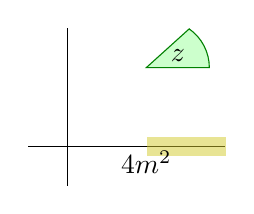
\begin{tikzpicture}
	\draw (-.5,0) -- (2,0);	\draw (0,-.5) -- (0,1.5);
	\filldraw[fill=green!20,draw=green!50!black] (1,1) -- +(8mm,0mm)
	arc [start angle=0, end angle=55, radius=6mm] -- cycle;
	\node at (1.4,1.15) {$z$};
	\node[fill=yellow!80!black,semitransparent,anchor=west,minimum width=1cm] at (1cm,0) {};
	\node at (1cm,-2mm) {$4m^2$};
\end{tikzpicture}

\end{document}